\chapter{Two-Flavor Quark--Meson Model}

The modern understanding of strongly interacting matter is rooted in
the development of QCD in the early 1970s.
With the discovery of asymptotic freedom, it became clear that the
fundamental degrees of freedom of the strong interaction are quarks
and gluons, whose effective interactions become weaker at large
momentum scales \cite{GrossWilczek1973,Politzer1973}. This insight
established QCD as a consistent microscopic theory and clarified that
the appropriate degrees of freedom describing strongly interacting
matter need not be the same in all physical regimes. While hadrons
emerge as the relevant low-energy excitations of QCD in vacuum and at
moderate densities, the theory itself is formulated in terms of quarks
and gluons, suggesting that quark-based descriptions may become more
appropriate at sufficiently high baryon densities.

QCD provides the fundamental description of the strong interaction,
but its direct application to cold and dense systems remains highly
challenging. The primary difficulty is that many nonperturbative
methods developed for QCD, including lattice QCD, are well suited to
high temperatures or vanishing baryon chemical potential, but become
problematic at finite density.
In particular, the fermion sign problem obstructs straightforward
numerical simulations in the regime of high baryon density and low
temperature. At finite baryon chemical potential, the mathematical
weight that appears in lattice QCD calculations is no longer positive
and can even become complex. This prevents its interpretation as a
probability distribution and makes standard Monte Carlo simulation
methods impractical \cite{TroyerWiese2005,DeForcrand2010}. As a result,
first-principles lattice calculations of dense QCD matter are
currently not available.

These difficulties have been recognized since the early development
of QCD and have motivated the construction of a variety of effective
models for strongly interacting matter
\cite{CollinsPerry1975,BaymChin1976}. Such models are not intended as
first-principles descriptions. Instead, they are designed to capture
selected physical features of QCD—most notably its symmetries and
symmetry-breaking patterns—while remaining computationally tractable.
In this way, effective models provide a practical framework for
exploring the qualitative behavior of dense matter in regimes where
direct applications of QCD are not yet possible.

The Quark--Meson model is one example of such an effective
description. Historically, it is closely related to the linear sigma
model introduced by Gell-Mann and Lévy as a theory of nucleons
interacting with scalar and pseudoscalar mesons
\cite{GellMannLevy1960}. In later developments, the fermionic degrees
of freedom were reinterpreted as quarks rather than nucleons, leading
to what is commonly referred to as the Quark--Meson model. In this
framework, quarks interact via Yukawa couplings with mesonic fields,
which serve as effective degrees of freedom encoding important
features of the strong interaction.

In its simplest form, the model contains two quark flavors, up and
down, coupled to a scalar field and an isotriplet of pseudoscalar
fields. The mesonic sector is constructed such that the model
reproduces the same global symmetry structure as QCD in the limit of
massless light quarks, where the Lagrangian is invariant under chiral
$SU(2)_L \times SU(2)_R$ transformations and different phases of
matter are distinguished by the realization of this symmetry in the
ground state.

At the same time, the model allows for both spontaneous and explicit
breaking of chiral symmetry. Spontaneous symmetry breaking arises
through the structure of the mesonic potential and is associated with
a nonvanishing vacuum expectation value of the scalar field. Explicit
symmetry breaking is introduced through terms that violate chiral
invariance at the level of the Lagrangian, mimicking the effect of
finite light-quark masses in QCD. As a consequence, a sharp chiral
phase transition present in the chiral limit is replaced by a smooth
crossover when explicit symmetry breaking is included.

The two-flavor Quark--Meson model has been widely employed as a
theoretical laboratory for investigating dense strongly interacting
matter, both on its own and in comparison with related chiral quark
models such as the Nambu--Jona-Lasinio model
\cite{Buballa2005}. Its relatively simple structure makes it
particularly well suited for mean-field treatments and for the
derivation of thermodynamic quantities starting from a Lagrangian
formulation \cite{SchaeferWambach2008}. For these reasons, it serves
as a natural starting point for introducing quark-based equations of
state.

Extensions of the model to include a third quark flavor are also
commonly studied. Three-flavor versions allow strange quarks to
participate and are often used in discussions of strange quark matter
and the possible appearance of strangeness at high density
\cite{SchaeferWambach2008,Buballa2005}. While such extensions introduce
additional parameters and physical uncertainties, they represent a
natural continuation of the two-flavor framework. In the present
chapter, however, we restrict attention to the two-flavor
Quark--Meson model, which already captures the essential conceptual
ingredients needed for the discussions that follow.


\section{From QCD to the Quark--Meson model}

The Quark--Meson model is constructed by isolating those features of
QCD that are expected to be most relevant for
the dynamics of light quarks at low and moderate energies, and by
building an effective field model that reproduces these features in
a simplified setting. In particular, the model is designed to reflect
the global symmetry structure of QCD and its characteristic pattern
of symmetry breaking, while the detailed microscopic dynamics
associated with gluon exchange are not retained explicitly
\cite{WeinbergQFT,PeskinSchroeder1995}.

QCD is a quantum field theory describing quarks interacting through
non-Abelian gauge fields. Its dynamics are defined by the QCD
Lagrangian density
\begin{equation}
\mathcal{L}_{\mathrm{QCD}}
= \sum_{f=1}^{N_f} \bar{q}_f^a\!\left(i\gamma^\mu D_\mu - m_f\right)\!q_f^a
- \frac{1}{4}\,G^A_{\mu\nu} G^{A\,\mu\nu},
\label{eq:LQCD}
\end{equation}
where $q_f^a$ denotes the quark field of flavor $f$ and color
$a=1,2,3$, $m_f$ is the corresponding bare quark mass parameter, and
$G^A_{\mu\nu}$ is the gluon field-strength tensor
\cite{PeskinSchroeder1995,Weinberg1995}.

The quark fields are Dirac spinors carrying both color and flavor
degrees of freedom. For later use, it is convenient to organize the
light-quark sector into a flavor multiplet. Restricting attention to
two flavors, one may write
\begin{equation}
q =
\begin{pmatrix}
u \\ d
\end{pmatrix},
\end{equation}
while keeping the explicit sum over flavors in
Eq.~\eqref{eq:LQCD}.

The interaction between quarks and gluons enters through the
gauge-covariant derivative
\begin{equation}
D_\mu \equiv \partial_\mu - i g\,A_\mu^A T^A,
\label{eq:covder}
\end{equation}
where $g$ is the QCD gauge coupling, $A_\mu^A$ are the gluon fields,
and $T^A$ are the generators of the color gauge group $SU(3)$ in the
fundamental representation. The index $A=1,\ldots,8$ labels the eight
generators (and therefore the eight gluon fields). With the standard
normalization one has
\begin{equation}
\mathrm{tr}(T^A T^B) = \frac{1}{2}\delta^{AB},
\end{equation}
and the generators satisfy the commutation relations
\begin{equation}
[T^A,T^B] = i f^{ABC} T^C,
\end{equation}
where $f^{ABC}$ are the structure constants of $SU(3)$
\cite{PeskinSchroeder1995}.

The final term in Eq.~\eqref{eq:LQCD} is the gluonic kinetic term. It
is written in terms of the non-Abelian field-strength tensor
\begin{equation}
G^A_{\mu\nu}
= \partial_\mu A_\nu^A - \partial_\nu A_\mu^A
+ g f^{ABC} A_\mu^B A_\nu^C .
\label{eq:Fmunu}
\end{equation}
The crucial difference from an Abelian gauge theory is the last term,
which is quadratic in the gauge fields. When inserted into
$G^A_{\mu\nu}G^{A\,\mu\nu}$ it produces three- and four-gluon
self-interactions. These self-interactions are a defining feature of
QCD and are ultimately responsible for its non-perturbative
behavior at low energies \cite{PeskinSchroeder1995,Weinberg1995}.

For our purposes it is useful to separate the ``matter part'' of QCD,
which involves quarks, from the purely gluonic part. Suppressing
explicit color indices, the quark contribution may be written
schematically as
\begin{equation}
\mathcal{L}_{\mathrm{q}}
= \bar{q}\,(i\gamma^\mu D_\mu - M)\,q,
\label{eq:Lqschematic}
\end{equation}
where $q$ denotes the quark field (with flavor components collected
into a multiplet) and $M$ is the mass matrix in flavor space. In the
two-flavor case $M=\mathrm{diag}(m_u,m_d)$. In this chapter we restrict
attention to the two lightest quark flavors, up and down, whose
bare masses are small compared to typical hadronic scales
\cite{PeskinSchroeder1995}.

Equation~\eqref{eq:Lqschematic} makes explicit the elements of QCD that
are relevant for the discussion that follows. In particular, it
exhibits the relativistic fermionic nature of the quark fields and the
structure of the mass term, both of which play a central role in the
symmetry properties of the theory. At this stage, we are not concerned
with the detailed dynamics generated by the gluonic self-interactions
in Eq.~\eqref{eq:Fmunu}, but rather with the global symmetries of the
light-quark sector and how these symmetries depend on the quark mass
matrix.

We begin by considering a global phase transformation of the quark
field,
\begin{equation}
q \rightarrow q' = e^{i\alpha} q ,
\qquad
\bar q \rightarrow \bar q' = \bar q e^{-i\alpha},
\label{eq:U1V}
\end{equation}
with constant $\alpha$. Since the phase factors cancel between $q$ and
$\bar q$, both the kinetic term and the mass term in the quark
Lagrangian are invariant under this transformation,
\begin{equation}
\bar q (i\gamma^\mu D_\mu - M) q
\;\longrightarrow\;
\bar q (i\gamma^\mu D_\mu - M) q .
\end{equation}
This symmetry is referred to as a global $U(1)_V$ symmetry and
corresponds to baryon number conservation. Importantly, $U(1)_V$
remains an exact symmetry of QCD even in the presence of finite quark
masses.

To uncover additional symmetry structures of the quark Lagrangian,
it is necessary to examine the spinor structure of the quark fields.
A key concept in this context is chirality. In relativistic quantum
field theory, the Dirac matrix $\gamma^5$ allows one to define the
projection operators
\begin{equation}
P_{L,R} = \frac{1}{2}(1 \mp \gamma^5),
\label{eq:projection_operators}
\end{equation}
where $\gamma^5$ satisfies $(\gamma^5)^2 = 1$, with $1$ understood as
the identity operator in Dirac space, and anticommutes with the Dirac
matrices $\gamma^\mu$. These operators possess several important
properties.

First, they are \emph{projection operators}, meaning that applying
them twice is equivalent to applying them once:
\begin{equation}
P_{L,R}^2
= \frac{1}{4}(1 \mp \gamma^5)(1 \mp \gamma^5)
= \frac{1}{4}(1 \mp 2\gamma^5 + (\gamma^5)^2)
= \frac{1}{2}(1 \mp \gamma^5)
= P_{L,R}.
\end{equation}

Second, the left- and right-handed projectors are \emph{orthogonal},
\begin{equation}
P_L P_R
= \frac{1}{4}(1 - \gamma^5)(1 + \gamma^5)
= \frac{1}{4}(1 - (\gamma^5)^2)
= 0,
\end{equation}
which implies that no spinor component can be simultaneously left-
and right-handed.

Third, the projectors satisfy the \emph{completeness relation},
\begin{equation}
P_L + P_R
= \frac{1}{2}(1 - \gamma^5) + \frac{1}{2}(1 + \gamma^5)
= 1,
\end{equation}
so that any Dirac spinor can be decomposed uniquely into left- and
right-handed parts.

Using the projection operators in \eqref{eq:projection_operators},
the quark field may be decomposed into its left- and right-handed
components,
\begin{equation}
q = q_L + q_R, \qquad
q_{L,R} = P_{L,R} q .
\end{equation}
This decomposition is always possible at the level of Dirac spinors
and reflects the fact that relativistic fermions admit states of
definite chirality.

We now apply the projection operators to the quark Lagrangian
\eqref{eq:Lqschematic} in order to express it in the left- and
right-handed basis defined above. We begin by examining the mass
term, which takes the form
\begin{equation}
\bar q M q
= \bar q_L M q_R + \bar q_R M q_L ,
\label{eq:qm_decomp}
\end{equation}
since terms of the form $\bar q_L M q_L$ and $\bar q_R M q_R$
vanish identically. The mass term therefore couples left- and
right-handed components explicitly. As long as $M \neq 0$, the two
chiralities are dynamically linked, and transformations acting
independently on $q_L$ and $q_R$ will in general not leave the
Lagrangian invariant.

For this reason, it is useful to consider the \emph{chiral limit},
$M \to 0$, in which the coupling between left- and right-handed
components disappears. In this limit, the quark Lagrangian reduces to
\begin{equation}
\mathcal{L}_{\mathrm{q}}
= \bar{q}_L\, i \gamma^\mu D_\mu\, q_L
+ \bar{q}_R\, i \gamma^\mu D_\mu\, q_R .
\label{eq:Lq_chiral}
\end{equation}
The left- and right-handed fields now appear in separate terms and are
no longer coupled to one another. They may therefore be transformed
independently without changing the form of the Lagrangian. This
decoupling is the origin of the enlarged symmetry structure of the
massless theory.

For two light quark flavors, the massless Lagrangian
\eqref{eq:Lq_chiral} is invariant under independent non-Abelian flavor
rotations of the left- and right-handed fields,
\begin{equation}
q_L \rightarrow U_L\, q_L,
\qquad
q_R \rightarrow U_R\, q_R,
\qquad
U_L, U_R \in SU(2)_{L,R},
\label{eq:abelian_rotations}
\end{equation}
which defines the global chiral symmetry group
$SU(2)_L \times SU(2)_R$ \cite{WeinbergQFT,ManoharGeorgi}. Explicitly,
an infinitesimal chiral transformation may be written as
\begin{equation}
q_L \rightarrow \left(1 + i \theta_L^i \frac{\tau^i}{2}\right) q_L,
\qquad
q_R \rightarrow \left(1 + i \theta_R^i \frac{\tau^i}{2}\right) q_R ,
\end{equation}
where $\tau^i$ are the Pauli matrices acting in flavor space and
$\theta_L^i$, $\theta_R^i$ are independent real parameters.

In addition to these non-Abelian flavor rotations, the chiral limit
also admits a global axial phase symmetry. Under an axial
transformation,
\begin{equation}
q \rightarrow q' = e^{i\beta \gamma^5} q ,
\qquad
\bar q \rightarrow \bar q' = \bar q e^{i\beta \gamma^5},
\label{eq:U1A}
\end{equation}
with constant $\beta$, the kinetic term remains invariant because
$\{\gamma^5,\gamma^\mu\}=0$. In terms of left- and right-handed
components, this transformation takes the form
\begin{equation}
q_L \rightarrow e^{-i\beta} q_L,
\qquad
q_R \rightarrow e^{+i\beta} q_R ,
\end{equation}
showing explicitly that $U(1)_A$ acts with opposite phases on $q_L$
and $q_R$.

For nonzero quark masses, the axial symmetry is explicitly broken.
Using \eqref{eq:qm_decomp}
one finds that the mass term is not invariant under the transformation
\eqref{eq:U1A}. Consequently, $U(1)_A$ is a symmetry only in the chiral
limit $M \to 0$.

At the quantum level, the axial $U(1)_A$ symmetry is further broken by
the axial anomaly, which arises from the non-invariance of the path
integral measure under axial transformations in the presence of gauge
fields \cite{Adler1969,BellJackiw1969}. Although the classical QCD
Lagrangian is invariant under $U(1)_A$ in the chiral limit, quantum
effects generate a nonvanishing divergence of the axial current,
proportional to $G^A_{\mu\nu}\tilde G^{A\,\mu\nu}$. This contribution
is associated with topologically nontrivial gluon configurations,
such as instantons, and leads to an explicit breaking of the
$U(1)_A$ symmetry \cite{tHooft1976}. 

As a consequence, $U(1)_A$ is not an exact symmetry of QCD even when
the quark masses vanish. Phenomenologically, this anomaly explains,
for example, why the $\eta'$ meson is much heavier than would be
expected from naive chiral symmetry arguments. In the present work,
we neglect the effects of the axial anomaly and focus on the
non-Abelian $SU(2)_L \times SU(2)_R$ symmetry, which plays the
central role in the construction of the Quark--Meson model.

Collecting the non-Abelian chiral rotations and the vector and axial
phase symmetries at the classical level, the global symmetry group of
the massless two-flavor quark Lagrangian may be written as
\begin{equation}
U(2)_L \times U(2)_R
\simeq SU(2)_L \times SU(2)_R \times U(1)_V \times U(1)_A .
\end{equation}
For small but nonzero light-quark masses, the chiral
$SU(2)_L \times SU(2)_R$ symmetry and the axial $U(1)_A$ symmetry are
explicitly broken, while the vector $U(1)_V$ symmetry associated with
baryon number conservation remains exact
\cite{WeinbergQFT,DonoghueGolowichHolstein}.

The two-flavor Quark--Meson model provides a minimal and explicit
realization of these requirements. It retains quark degrees of
freedom and implements chiral symmetry directly at the level of the
Lagrangian, while introducing additional mesonic fields that allow
the pattern of chiral symmetry breaking to be represented
explicitly. The strength of both spontaneous and explicit symmetry
breaking is governed by a small set of parameters in the mesonic
sector, making their effects straightforward to identify and vary.
The structure of the model is therefore fixed primarily by symmetry
considerations, which constrain the form of the allowed
interaction terms.

The simplest fermion bilinear that couples left- and right-handed
fields is $\bar{q}_L q_R$ (and its Hermitian conjugate). In order to
construct a chirally invariant interaction, this bilinear must be
multiplied by a bosonic field that transforms appropriately under
$SU(2)_L \times SU(2)_R$. This motivates the introduction of a set of
bosonic fields that carry the same chiral transformation properties
as the quark bilinear $\bar{q}_R q_L$. Historically, this idea traces
back to the linear sigma model of Gell-Mann and L\'evy
\cite{GellMannLevy1960}.

Concretely, one introduces a real scalar field $\sigma$ and a triplet
of real pseudoscalar fields
$\boldsymbol{\pi} = (\pi_1,\pi_2,\pi_3)$. These fields represent
color-singlet mesonic degrees of freedom and are to be interpreted as
effective hadronic excitations of QCD at low energies. In this sense,
they play a role analogous to protons and neutrons in ordinary
low-temperature nuclear matter: they are not fundamental quark and
gluon fields, but composite, confined objects that constitute the
relevant physical degrees of freedom in the infrared regime.

In particular, the pion fields correspond to the light pseudoscalar
mesons associated with spontaneous chiral symmetry breaking, while the
$\sigma$ field describes the corresponding scalar excitation. They do
not appear as elementary fields in the QCD Lagrangian, but emerge as
collective modes of the strongly interacting quark–gluon system. Their
masses are therefore of hadronic origin, set by the scale of chiral
symmetry breaking and confinement, rather than by the bare quark mass
parameters of QCD.

It is convenient to organize the mesonic fields into a matrix-valued
field in flavor space,
\begin{equation}
\Sigma = \sigma + i \boldsymbol{\tau}\cdot\boldsymbol{\pi},
\label{eq:sigma_def}
\end{equation}
where $\boldsymbol{\tau}$ denotes the Pauli matrices. The usefulness of
this construction becomes apparent when considering chiral
transformations. Under a global $SU(2)_L \times SU(2)_R$ symmetry
transformation, the quark fields transform according to \eqref{eq:abelian_rotations}.
Requiring the interaction between quarks and
mesons to respect the same symmetry uniquely fixes the transformation
property of the mesonic field to be
\begin{equation}
\Sigma \rightarrow U_L\, \Sigma\, U_R^\dagger .
\end{equation}
With this assignment, the combination
$\bar{q}_L \Sigma q_R + \bar{q}_R \Sigma^\dagger q_L$
is invariant under $SU(2)_L \times SU(2)_R$ transformations. This
provides a natural and symmetry-consistent way of coupling quark
fields to the mesonic degrees of freedom.

\section{The Two-Flavor Quark-Meson Lagrangian}
Having identified the allowed interaction terms, one may now
construct the Lagrangian density of the two-flavor Quark--Meson model.
It consists of three distinct parts: a fermionic kinetic term, a
chirally invariant Yukawa interaction between quarks and mesons, and
a purely mesonic sector describing the dynamics of the bosonic fields,
\begin{equation}
\mathcal{L}_{\mathrm{QM}} =
\bar{q}\left(i \gamma^\mu \partial_\mu
- g \left[\sigma + i \gamma^5 \boldsymbol{\tau}\cdot\boldsymbol{\pi}
\right]\right) q
+ \mathcal{L}_{\mathrm{mes}} .
\end{equation}
Here $g$ is a Yukawa coupling constant. The appearance of the
$\gamma^5$ matrix reflects the pseudoscalar nature of the pion fields
and ensures the correct transformation properties under parity and
chiral symmetry.

The matrix-valued field $\Sigma$, defined in \eqref{eq:sigma_def},
transforms under global $SU(2)_L \times SU(2)_R$ rotations as
\begin{equation}
\Sigma \;\longrightarrow\; U_L \Sigma U_R^\dagger ,
\qquad
U_L \in SU(2)_L, \quad U_R \in SU(2)_R .
\end{equation}
Chiral invariants must therefore be constructed from quantities that
are unchanged under this transformation. Since
\begin{equation}
\Sigma^\dagger \Sigma
\;\longrightarrow\;
U_R (\Sigma^\dagger \Sigma) U_R^\dagger ,
\end{equation}
its trace is invariant,
\begin{equation}
\mathrm{Tr}(\Sigma^\dagger \Sigma)
\;\longrightarrow\;
\mathrm{Tr}(\Sigma^\dagger \Sigma),
\end{equation}
where we have used the cyclic property of the trace.
More generally, all invariant operators in the mesonic sector can be
constructed from traces of products of $\Sigma$ and $\Sigma^\dagger$.

The mesonic kinetic term is uniquely fixed by this symmetry structure
and can be written compactly as
\begin{equation}
\mathcal{L}_{\mathrm{kin}}^{\mathrm{mes}}
=
\frac{1}{2}\,\mathrm{Tr}\!\left(
\partial_\mu \Sigma^\dagger \partial^\mu \Sigma
\right),
\end{equation}
which is invariant under global chiral rotations.

The remaining freedom lies in the choice of the mesonic potential.
Locality and renormalizability in four spacetime dimensions restrict
the potential to operators of mass dimension four or less.
Furthermore, the potential must be constructed from chiral invariants,
which limits the allowed structures to traces of products of
$\Sigma^\dagger \Sigma$.

At quadratic order, the only invariant is
\begin{equation}
\mathrm{Tr}(\Sigma^\dagger \Sigma)
=
\sigma^2 + \boldsymbol{\pi}^2 .
\end{equation}
At quartic order, two seemingly independent invariants can be formed,
\begin{equation}
\left[\mathrm{Tr}(\Sigma^\dagger \Sigma)\right]^2,
\qquad
\mathrm{Tr}(\Sigma^\dagger \Sigma \Sigma^\dagger \Sigma).
\end{equation}
For $2\times2$ matrices, however, these structures are not
independent. The Cayley--Hamilton theorem implies that any power of a
$2\times2$ matrix can be expressed in terms of the matrix itself and
the identity \cite{HornJohnson2012, PeskinSchroeder1995}.
As a consequence, the two quartic invariants above are
proportional to one another in the two-flavor case. Only a single
independent quartic coupling is therefore required.

This simplification is special to $SU(2)$. For three flavors, where
$\Sigma$ is a $3\times3$ matrix transforming under
$SU(3)_L \times SU(3)_R$, the two quartic structures are 
independent. In that case the Cayley--Hamilton relation for $3\times3$
matrices does not reduce one quartic invariant to the other, and both
must be included in the most general renormalizable potential.

Including also a linear term that explicitly breaks chiral symmetry,
the most general renormalizable mesonic potential consistent with
$SU(2)_L \times SU(2)_R$ symmetry at tree level may be written as
\begin{equation}
V(\sigma,\boldsymbol{\pi}) =
\frac{m^2}{2}(\sigma^2 + \boldsymbol{\pi}^2)
+ \frac{\lambda}{4}(\sigma^2 + \boldsymbol{\pi}^2)^2
- h\,\sigma .
\label{eq:mesonic_potential}
\end{equation}
The parameters $m^2$ and $\lambda$ determine the overall shape of the
potential. The linear term proportional to $h$ explicitly breaks
chiral symmetry and mimics the effect of finite light-quark masses in
QCD. In the chiral limit $h \to 0$, the potential depends only on the
invariant combination $\sigma^2 + \boldsymbol{\pi}^2$ and exhibits the
degenerate Mexican-hat structure. For $h \neq 0$, the term $-h\sigma$
tilts the hat, lifting the degeneracy of the minima and selecting a
unique vacuum configuration.

Each term in the Quark--Meson Lagrangian thus has a clear origin. The
Yukawa interaction provides a chirally invariant mechanism for
generating effective quark masses, the kinetic term describes
propagating mesonic degrees of freedom, and the potential encodes the
possibility of both spontaneous and explicit symmetry breaking. The
structure of the model is therefore fixed almost entirely by symmetry
and renormalizability, in accordance with the general philosophy of
effective field theory \cite{WeinbergEFT}.

To analyze the vacuum structure we work at tree level and neglect
quantum fluctuations. The mesonic fields are decomposed into a
spacetime-independent background part and fluctuations,
\begin{equation}
\sigma(x) = \sigma_0 + \tilde{\sigma}(x),
\qquad
\boldsymbol{\pi}(x) = \boldsymbol{\pi}_0 + \tilde{\boldsymbol{\pi}}(x).
\label{eq:quantum_and_constant}
\end{equation}
The constants $\sigma_0$ and $\boldsymbol{\pi}_0$ denote the classical
background fields, while $\tilde{\sigma}(x)$ and
$\tilde{\boldsymbol{\pi}}(x)$ describe fluctuations about the vacuum.
By definition, the background fields coincide with the vacuum
expectation values,
\begin{equation}
\langle \sigma \rangle = \sigma_0,
\qquad
\langle \boldsymbol{\pi} \rangle = \boldsymbol{\pi}_0 .
\end{equation}
In the classical approximation adopted here, the fluctuations are
ignored when determining the ground state. The vacuum configuration is
therefore obtained by minimizing the classical potential
$V(\sigma_0,\boldsymbol{\pi}_0)$ with respect to the background fields.

In the chiral limit $h=0$, the stationary conditions follow from
\begin{equation}
\frac{\partial V}{\partial \sigma_0}
= m^2 \sigma_0 + \lambda \sigma_0(\sigma_0^2 + \boldsymbol{\pi}_0^2)
= 0 ,
\end{equation}
with analogous equations for the pion components. Two qualitatively
distinct regimes arise, depending on the sign of $m^2$.

If $m^2>0$, the potential has a unique minimum at
\begin{equation}
\sigma_0 = 0, \qquad \boldsymbol{\pi}_0=0 .
\end{equation}
The vacuum expectation values therefore vanish, and the ground state
is invariant under the full $SU(2)_L \times SU(2)_R$ symmetry of the
Lagrangian. In this case the symmetry is realized in the
Wigner--Weyl (linear) mode \cite{WeinbergQFT}: the symmetry generators
annihilate the vacuum, the spectrum organizes into chiral multiplets,
and no additional massless modes appear.

If $m^2<0$, the stationary condition becomes
\begin{equation}
\sigma_0^2 + \boldsymbol{\pi}_0^2
= -\frac{m^2}{\lambda},
\end{equation}
so that the minima form a three-dimensional sphere in field space.
Since the four real fields
$(\sigma_0,\pi_{0,1},\pi_{0,2},\pi_{0,3})$ span $\mathbb{R}^4$,
the set of minima defines a three-sphere
\begin{equation}
S^3 \subset \mathbb{R}^4 ,
\end{equation}
known as the \emph{vacuum manifold}. The vacuum is therefore not
unique, but consists of a degenerate family of ground states related
by chiral transformations.

Figure~\ref{fig:mexican_hat} illustrates this structure in the chiral
limit $h \to 0$. For visualization only a single pion direction is
shown, so the vacuum manifold appears as a circle $S^1$. In the full
two-flavor theory, however, the pion field has three components and
the true vacuum manifold is the three-sphere $S^3$ described above.

The geometry of the vacuum manifold determines the spectrum of small
fluctuations. Tangential fluctuations — motion along $S^3$ — leave the
value of the potential unchanged to quadratic order. The potential has
vanishing curvature in these directions, which implies massless modes
in the chiral limit. These tangential excitations correspond to the
three pion fields and reflect the three broken axial generators.

In contrast, radial fluctuations change the value of
$\sigma_0^2 + \boldsymbol{\pi}_0^2$ and move the system away from the
vacuum manifold. The potential has nonzero curvature in this direction,
which generates a finite mass for the radial fluctuation $\tilde{\sigma}(x)$.

\begin{figure}[ht]
\centering
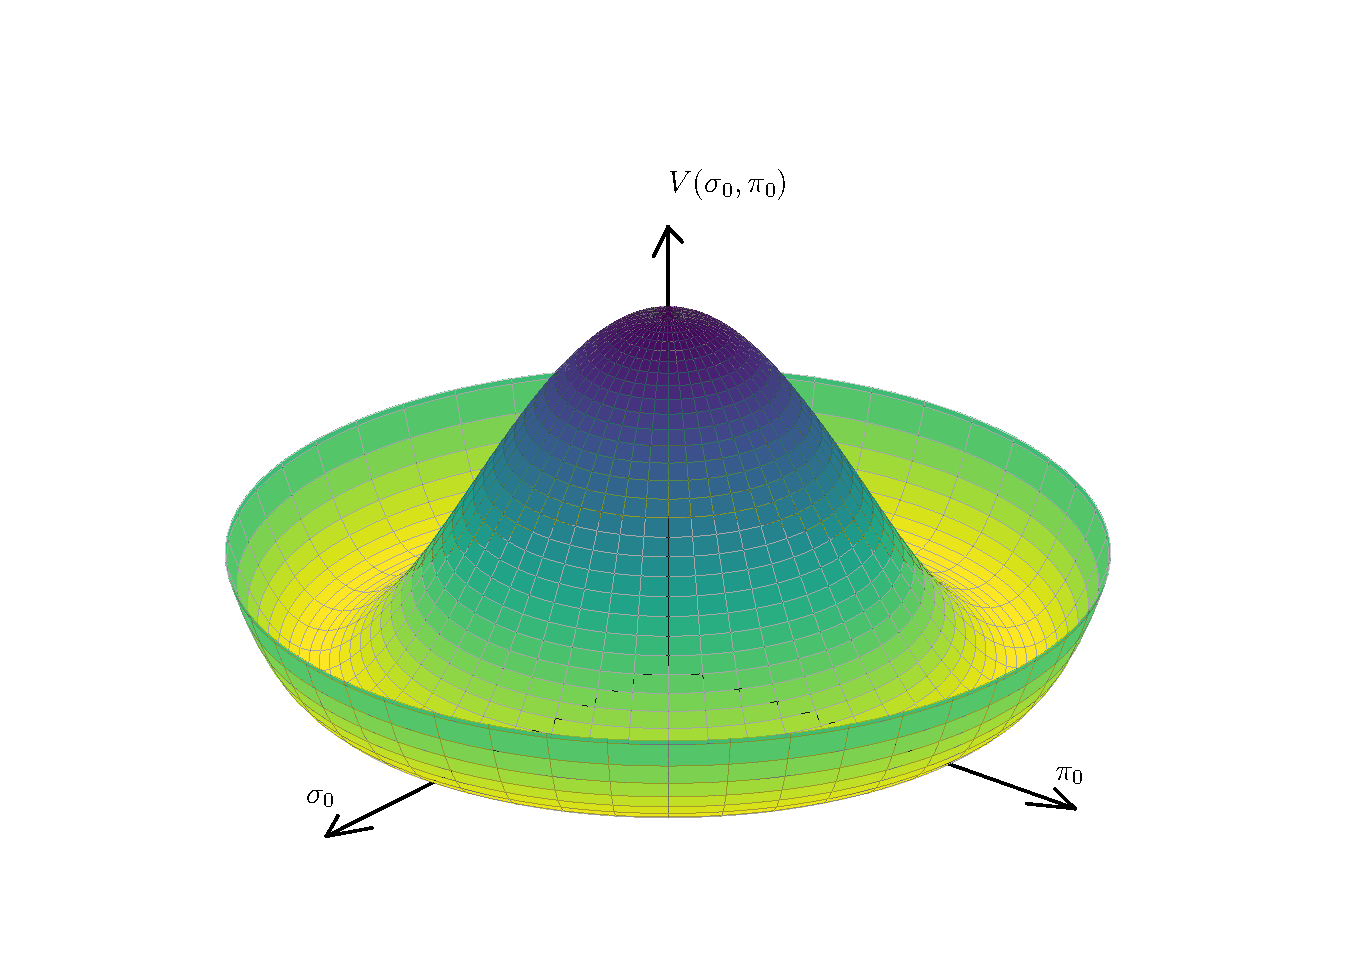
\includegraphics[width=0.75\textwidth]{figures/quark_meson/mexican_hat.pdf}
\caption{Mesonic potential for $m^2<0$ and $h=0$. The continuous valley
of degenerate minima reflects spontaneous symmetry breaking.}
\label{fig:mexican_hat}
\end{figure}

Although the Lagrangian remains invariant under
$SU(2)_L \times SU(2)_R$, a specific ground state must be selected.
Without loss of generality one may choose the vacuum to lie entirely
in the $\sigma_0$ direction,
\begin{equation}
\sigma_0 = v,
\qquad
\boldsymbol{\pi}_0 = 0.
\end{equation}
Since all points on the vacuum manifold are related by chiral
transformations, this choice corresponds merely to a convenient
orientation in field space. The constant $v$ therefore denotes the
vacuum expectation value of the scalar field in this chosen basis,
$\langle \sigma \rangle = v$.

In the chiral limit $h=0$, the magnitude satisfies
\begin{equation}
v^2 = -\frac{m^2}{\lambda}.
\end{equation}
The parameter $v$ serves as an order parameter for chiral symmetry
breaking: $v \neq 0$ signals the broken phase, whereas $v=0$
corresponds to the symmetric phase.

The chosen vacuum is invariant only under transformations with
$U_L = U_R$, forming the vector subgroup $SU(2)_V$. The symmetry-breaking
pattern is therefore
\begin{equation}
SU(2)_L \times SU(2)_R
\longrightarrow
SU(2)_V .
\end{equation}
Since the original group has six generators and the unbroken subgroup
has three, three generators are spontaneously broken.

Goldstone's theorem states that in a relativistic, Lorentz-invariant
quantum field theory, every spontaneously broken continuous global
symmetry generator gives rise to a massless scalar mode in the
spectrum \cite{Goldstone1961,
GoldstoneSalamWeinberg1962,WeinbergQFT}. For the breaking pattern
$SU(2)_L \times SU(2)_R \to SU(2)_V$, this yields three massless
pion modes in the chiral limit. The fluctuation $\tilde{\sigma}(x)$
corresponds to the radial excitation and is massive already at tree level.

When explicit symmetry breaking is included ($h\neq0$), the linear
term tilts the potential and removes the degeneracy of the vacuum,
selecting a unique minimum along the $\sigma_0$ direction, as shown in
Fig.~\ref{fig:tilt_profile}.

\begin{figure}[ht]
\centering
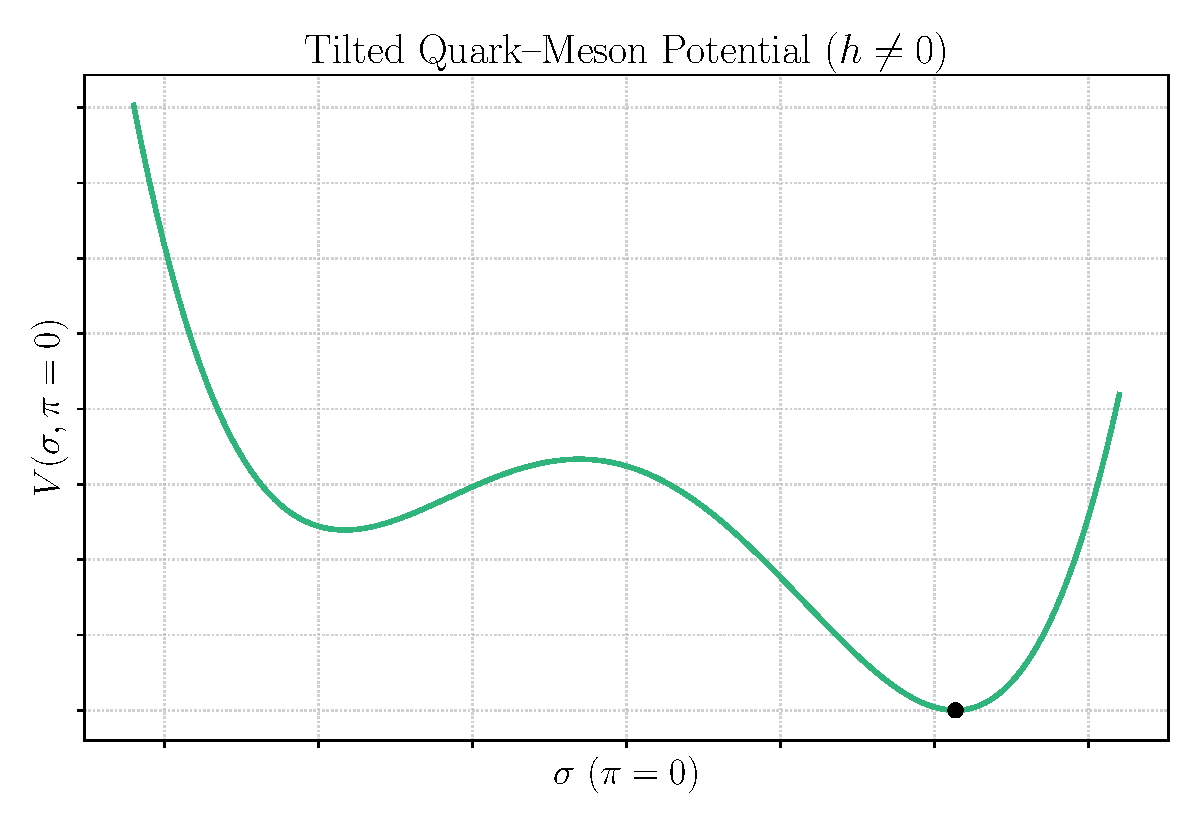
\includegraphics[width=0.75\textwidth]{figures/quark_meson/tilt_profile.pdf}
\caption{Potential profile along the $\mathbf{\pi}_0=0$ direction for $h\neq0$.
The degeneracy of the Mexican-hat minimum is lifted.}
\label{fig:tilt_profile}
\end{figure}

When explicit symmetry breaking is included ($h\neq0$), the vacuum
expectation value $v$ is determined from the stationary (tree-level
gap) equation
\begin{equation}
\left.\frac{\partial V}{\partial \sigma_0}\right|_{\sigma_0=v,\,
\boldsymbol{\pi}_0=0}
=
m^2 v + \lambda v^3 - h
=
0 .
\label{eq:gap_equation}
\end{equation}
This condition ensures that the linear terms in the fluctuation fields
vanish when the scalar field is expanded about the vacuum.

For the pion fields one finds
\begin{equation}
m_\pi^2
=
\left.
\frac{\partial^2 V}{\partial \pi_{0,i}^2}
\right|_{\sigma_0=v,\boldsymbol{\pi}_0=0}
=
m^2 + \lambda v^2 .
\label{eq:mpi_intermediate}
\end{equation}
At this stage the mass still depends explicitly on $m^2$ and $v$.
However, using the gap equation \eqref{eq:gap_equation} one may rewrite
\begin{equation}
m^2 + \lambda v^2 = \frac{h}{v},
\end{equation}
so that the squared pion mass takes the compact form
\begin{equation}
m_\pi^2 = \frac{h}{v}.
\label{eq:mpi_final}
\end{equation}

This expression makes the role of explicit symmetry breaking
transparent. In the strict chiral limit $h\to0$, the stationary
condition implies
\begin{equation}
m^2 + \lambda v^2 = 0 ,
\end{equation}
and therefore
\begin{equation}
m_\pi^2 = 0 .
\end{equation}
The pions are then exact massless Goldstone bosons, corresponding to
fluctuations tangential to the vacuum manifold.

For nonzero $h$, the degeneracy of the vacuum is lifted and the
potential acquires a small curvature along the previously flat
directions. The pion fields therefore become massive, but remain light
if $h$ is small. They are thus identified as pseudo-Goldstone bosons.

The squared mass of the radial fluctuation $\tilde{\sigma}$ follows from
\begin{equation}
m_\sigma^2
=
\left.
\frac{\partial^2 V}{\partial \sigma_0^2}
\right|_{\sigma_0=v,\boldsymbol{\pi}_0=0}
=
m^2 + 3\lambda v^2 .
\end{equation}
Unlike the pion mass, this expression does not vanish in the chiral
limit. $\tilde{\sigma}$ describes radial fluctuations orthogonal to
the vacuum manifold, where the potential has nonzero curvature already
at $h=0$. Consequently, the radial fluctuation $\tilde{\sigma}(x)$ 
remains massive even in the exactly symmetric Lagrangian.

The mass spectrum therefore directly reflects the geometry of the
vacuum manifold: tangential directions correspond to (pseudo-)Goldstone
modes, while the radial direction corresponds to a massive scalar
excitation.

The nonvanishing vacuum expectation value also has direct consequences
for the quark sector. 
After choosing the vacuum $\sigma_0=v$, the decomposition is
$\sigma(x)=v+\tilde{\sigma}(x)$, and the Yukawa interaction term becomes
\begin{equation}
- g \bar q \sigma q
=
- g v \bar q q
- g \bar q \tilde{\sigma} q .
\end{equation}
The first term has precisely the structure of a fermion mass term, so
that the quark fields acquire an effective mass
\begin{equation}
M_q = g v .
\end{equation}
Importantly, this mass is not inserted by hand in the Lagrangian. The
Yukawa interaction itself is chirally invariant, but once the field
develops a nonzero expectation value $v$, the interaction generates a
term proportional to $\bar q q$, which is not invariant under axial
transformations. In this way, the symmetry of the Lagrangian is
preserved, while the symmetry of the vacuum induces a mass for the
quarks.

The quantity $v$ therefore acts as an order parameter not only for the
mesonic sector but also for the fermionic degrees of freedom. When
$v \neq 0$, chiral symmetry is spontaneously broken and the quarks
behave as massive constituent particles. When $v \to 0$, corresponding
to the symmetric phase, the dynamically generated mass vanishes and
the quarks become effectively massless in the chiral limit. This
mechanism provides a concrete realization of how spontaneous chiral
symmetry breaking generates constituent quark masses, in close analogy
with the role played by the quark condensate $\langle \bar q q \rangle$
in QCD \cite{Nambu1961,WeinbergQFT}.

In a thermodynamic setting, the vacuum expectation value generally
depends on temperature and baryon chemical potential. The medium
dependence of $v$ therefore translates directly into a medium-dependent
quark mass $M_q = g v(T,\mu)$, which plays a central role in determining
the equation of state of the model.
